\section{Methodology \& Implementation} 

\begin{frame}[label=methodologyimplementation]{Methodology and Implementation}

\begin{block}{Objective}
    \begin{itemize}
        \item Forecast next-day WDAY stock prices using LSTM and LSTM-BiGRU models
        \item Assess robustness in volatile, mid-cap stock environments
    \end{itemize}
\end{block}

\note{
We now present both the methodological framework and its practical implementation, covering data 
preparation, model building, and evaluation.
}
\end{frame}


\begin{frame}[label=timeline, shrink]{Project Timeline: From Data to Prediction}

\begin{center}
\centerresizebox{
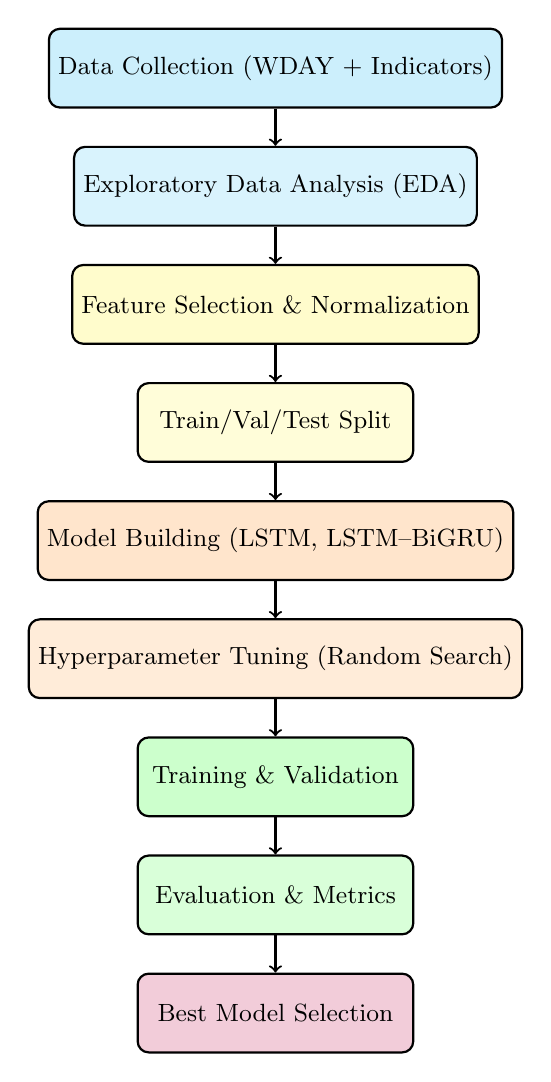
\begin{tikzpicture}[node distance=1.5cm, every node/.style={draw, rectangle, rounded corners, minimum width=3.5cm, minimum height=1cm, font=\small, align=center}, every path/.style={draw, thick, ->}]

% Nodes
\node[fill=cyan!20]  (start) {Data Collection (WDAY + Indicators)};
\node[fill=cyan!15] (eda) [below of=start] {Exploratory Data Analysis (EDA)};
\node[fill=yellow!20] (feature) [below of=eda] {Feature Selection \& Normalization};
\node[fill=yellow!15] (split) [below of=feature] {Train/Val/Test Split};
\node[fill=orange!20] (build) [below of=split] {Model Building (LSTM, LSTM–BiGRU)};
\node[fill=orange!15] (tuning) [below of=build] {Hyperparameter Tuning (Random Search)};
\node[fill=green!20] (train) [below of=tuning] {Training \& Validation};
\node[fill=green!15] (evaluation) [below of=train] {Evaluation \& Metrics};
\node[fill=purple!20] (end) [below of=evaluation] {Best Model Selection};

% Arrows
\draw (start) -- (eda);
\draw (eda) -- (feature);
\draw (feature) -- (split);
\draw (split) -- (build);
\draw (build) -- (tuning);
\draw (tuning) -- (train);
\draw (train) -- (evaluation);
\draw (evaluation) -- (end);

\end{tikzpicture}
}
\end{center}

\note{
This timeline summarizes the end-to-end methodology, beginning with WDAY data collection and ending with selecting the best-performing model after evaluation.
Each step feeds logically into the next, ensuring a consistent experimental pipeline.
}
\end{frame}

\begin{frame}[label=datacollectioneda]{Data Collection and Initial Analysis}

\begin{block}{Sources}
    \begin{itemize}
        \item WDAY stock data via Twelve Stock Market API
        \item 10 years of daily OHLCV prices (2014–2025)
        \item Technical indicators for trend, momentum, volatility, and volume
    \end{itemize}
\end{block}

\begin{alertblock}{Exploratory Data Analysis (EDA)}
    2,820 clean daily records analyzed for descriptive statistics and volatility behavior (a decent but relatively small dataset by deep learning standards).
\end{alertblock}

\note{
We collected 10 years of daily WDAY data, enabling a robust view of long-term economic cycles.
Technical indicators were calculated, offering momentum, trend, and volatility insights.
The EDA showed that the dataset was clean and stable, providing a strong basis for modeling.
}
\end{frame}

\begin{frame}[label=datastructure,shrink]{Dataset Overview: Features and Indicators}
\begin{table}
\centering
\caption{Categories of Features in the WDAY Dataset}
\label{tab:datasetstructure}
\renewcommand{\arraystretch}{1.7} 
\begin{tabular}{p{2cm}p{12.5cm}}
\hline
\textbf{Category} & \textbf{Description} \\
\hline\hline
\textbf{Pricing} & Includes daily Open, High, Low, Close, and Volume (OHLCV) 
values, serving as the \alert{foundation for tracking stock performance}. \\
\textbf{Trend} & Measure the overall market direction, 
\alert{helping to identify uptrends, downtrends}, or sideways movements. \\
\textbf{Momentum} & Evaluate the \alert{speed and strength of price movements},
providing insights into potential trend reversals and overbought/oversold 
conditions. \\
\textbf{Volatility} & Assess market risk and \alert{price fluctuations}, identifying 
potential breakouts and periods of stability. \\
\textbf{Volume} & Analyze trading activity to confirm price trends and \alert{detect accumulation (buying) or distribution (selling) behavior}. \\
\hline
\end{tabular}
\end{table}

\note{
The dataset is structured around five major feature categories.
Pricing Data (OHLCV) forms the base, while Trend, Momentum, Volatility, and Volume indicators enrich the inputs.
These indicators offer critical signals about market behavior, improving the model's ability to forecast stock price movements.
Using multiple indicator types ensures the model captures various dimensions of stock performance, not just raw prices.
}
\end{frame}

\begin{frame}[label=datawindow,shrink]{Why 10 Years of Daily Data?}

\small
\begin{table}
\centering
\caption{Recommended Data Windows and Interval for Stock Price Prediction}
\label{tab:data-window}
\renewcommand{\arraystretch}{1.7} 
\begin{tabular}{p{2cm}p{2cm}p{2cm}p{4cm}}
\hline
\textbf{Study} & \textbf{Window} & \textbf{Interval} & \textbf{Use Case} \\
\hline\hline
\parencite{shaban2024SMPDL} & 2 Years & Every Minute & High-frequency trading (HFT) \\
\parencite{guo2024LSTMStock} & 125 days & Every Minute & HFT bursts, micro-movement learning \\
\parencite{chang2024StockPrediction}, \parencite{nabipour2020DeepLearning} & 
\alert{10 Years} & \alert{Daily} & \alert{Medium-term forecasting} \\
\hline
\end{tabular}
\end{table}

\note{
Here’s the reasoning behind our choice:

- \textbf{Shaban et al. (2024)} used minute-level data for HFT. While very precise, it is extremely noisy, requires heavy computation, and is often unsuitable for broader trend forecasting.
- \textbf{Guo et al. (2024)} also used minute data but only over short bursts (125 days). Again, good for micro-movement analysis, but lacks the ability to capture economic cycles or mid-term patterns.
- \textbf{Chang (2024)} and \textbf{Nabipour (2020)} chose 10 years of daily data. This approach captures complete economic cycles, offers broader trend detection, and aligns better with end-of-day price prediction goals.

Thus, our methodology adopts a daily, 10-year window to focus on generalizable, meaningful stock trends rather than short-term noise.
}
\end{frame}

\begin{frame}[label=datasetsplit, shrink]{Dataset Split Strategy}

\small

\begin{block}{Why Time-Based Splitting?}
\begin{itemize}
    \item Time-series data must maintain chronological order to avoid data leakage.
    \item Ensures that the model only uses \textbf{past} information to predict the \textbf{future}.
    \item Aligns with best practices in financial forecasting research~\parencite{chang2024StockPrediction, guo2024LSTMStock}.
\end{itemize}
\end{block}

\vspace{0.5em}
{\footnotesize
\begin{equation}
\label{eq:dataset_split_dates}
\underbrace{X_{\text{2014-01-02}}, \dots, X_{\text{2021-11-08}}}_{\text{Training Data (75\%)}} 
\quad
\underbrace{X_{\text{2021-11-09}}, \dots, X_{\text{2023-07-20}}}_{\text{Validation Data (15\%)}} 
\quad
\underbrace{X_{\text{2023-07-21}}, \dots, X_{\text{2025-03-28}}}_{\text{Test Data (15\%)}} 
\end{equation}
}
\note{
In financial forecasting, preserving the temporal structure is crucial.

We split the dataset chronologically:
\begin{itemize}
    \item 75\% for training — covering over 7 years of historical patterns.
    \item 15\% for validation — tuning hyperparameters.
    \item 15\% for testing — strictly future, unseen data from volatile periods.
\end{itemize}
The chronological split avoids any future data leakage into training and reflects real-world stock prediction challenges.
}
\end{frame}



\begin{frame}[label=featurescalingworkflow]{Feature Scaling Workflow: How We Prevent Leakage}

\small

\begin{block}{Scaler Fitting and Application}
\begin{itemize}
    \item \textbf{MinMaxScaler} is \textbf{fit only on the Training Set}.
    \item The learned scaling parameters ($x_{\min}$, $x_{\max}$) are reused for Validation and Test Sets.
    \item Ensures consistent input distribution and prevents leakage.
\end{itemize}
\end{block}

\begin{alertblock}{Why MinMaxScaler for LSTM?}
MinMaxScaler ensures that inputs match LSTM activation functions (tanh/sigmoid), improving training stability, convergence speed, and balancing feature influence
~\parencite{shaban2024SMPDL,phuoc2024StockPrediction}.
\end{alertblock}

\note{
In financial time-series forecasting, it is essential to avoid data leakage when scaling features.

We fit the MinMaxScaler exclusively on the Training Set. 
This ensures that the scaler parameters are only influenced by past information.
Then, we reuse these parameters when scaling the Validation and Test sets.

This approach mirrors a real-world scenario where future data is unknown during model training, ensuring that model performance evaluation is realistic and unbiased.
}
\end{frame}



